%%%%%%%%%%%%%%%%%%%%%%%%%%%%%%%%%%%%%%%%%
% a0poster Landscape Poster
% LaTeX Template
% Version 1.0 (22/06/13)
%
% The a0poster class was created by:
% Gerlinde Kettl and Matthias Weiser (tex@kettl.de)
%
% This template has been downloaded from:
% http://www.LaTeXTemplates.com
%
% License:
% CC BY-NC-SA 3.0 (http://creativecommons.org/licenses/by-nc-sa/3.0/)
%
%%%%%%%%%%%%%%%%%%%%%%%%%%%%%%%%%%%%%%%%%

%----------------------------------------------------------------------------------------
%    PACKAGES AND OTHER DOCUMENT CONFIGURATIONS
%----------------------------------------------------------------------------------------

\documentclass[a0,portrait]{a0poster}

\usepackage{multicol} % This is so we can have multiple columns of text side-by-side
\columnsep=100pt % This is the amount of white space between the columns in the poster
\columnseprule=3pt % This is the thickness of the black line between the columns in the poster

\usepackage{microtype}
\usepackage{vwcol}
\usepackage{lipsum}
\usepackage[hidelinks]{hyperref}
\usepackage{multirow}

\usepackage[svgnames]{xcolor} % Specify colors by their 'svgnames', for a full list of all colors available see here: http://www.latextemplates.com/svgnames-colors

%\usepackage{times} % Use the times font
%\usepackage{palatino} % Uncomment to use the Palatino font

\usepackage[sc]{mathpazo}
\linespread{1.05}         % Palladio needs more leading (space between lines)
\usepackage[T1]{fontenc}

\usepackage{graphicx} % Required for including images
\graphicspath{{fig/}} % Location of the graphics files
\usepackage{booktabs} % Top and bottom rules for table
\usepackage[font=small,labelfont=bf]{caption} % Required for specifying captions to tables and figures
\usepackage{amsfonts, amsmath, amssymb, mathrsfs} % For math fonts, symbols and environments
\usepackage{wrapfig} % Allows wrapping text around tables and figures
\usepackage{changepage}   % Adjust boundary temporarily
\usepackage{caption}
\usepackage[nottoc,numbib]{tocbibind}
\usepackage{biblatex}
\usepackage[normalem]{ulem}
%\captionsetup[table]{skip=.5cm} % Adjust spacing between caption and table

\DeclareMathOperator*{\argmin}{argmin}
\DeclareMathOperator*{\argmax}{argmax}

\newcommand{\eat}[1]{}
\newcommand{\secmoveup}{\vspace{-1cm}}
\newcommand{\textmoveup}{\vspace{-.5cm}}
\newcommand{\captionmoveup}{\vspace{-.5cm}}
\newcommand{\eqmoveup}{\vspace{-.3cm}}

\setlength{\columnseprule}{0pt}

\bibliography{ref.bib}

\begin{document}

%----------------------------------------------------------------------------------------
%    POSTER HEADER
%----------------------------------------------------------------------------------------

\begin{adjustwidth}{-.3cm}{}
\begin{tabular}{lr}
\Huge
\color{NavyBlue} \textbf{Quantile Regression Upper Confidence Bound} \color{Black}
&
\multirow{3}{*}{
\includegraphics[height=4.2cm]{anu-logo.jpg}\hspace{.5cm}
\includegraphics[height=4.2cm]{data61-logo.jpg}} \\
\vspace{.1cm} & \\
\hspace{.1cm}\LARGE\textbf{\it Mengyan Zhang, Cheng Soon Ong}, Australian National University \& Data61
\end{tabular}
\end{adjustwidth}

\vspace{1.5cm} % A bit of extra whitespace between the header and poster content

%----------------------------------------------------------------------------------------

\begin{multicols}{2} % This is how many columns your poster will be broken into, a poster with many figures may benefit from fewer columns whereas a text-heavy poster benefits from more

%----------------------------------------------------------------------------------------
% column 1
%----------------------------------------------------------------------------------------

\section{Problem Statement and Background}
\vspace{-.2cm}

\noindent
Many applications require optimizing an unknown, noisy function that is expensive to evaluate, which can be formalized as a multiarmed bandit problem. Consider the problem of sequential optimizing an unknown reward function $f: D \rightarrow \mathbb{R}$. In each round t, we choose a point $x_t \in D$ and learn its function value with noise: $y_t = f(x_t) + \epsilon_t$. The goal is to maximise the cumulative rewards $\sum_{t=1}^T f(x_t)$ and thus to perform $x_\ast = \argmax_{x \in D} f(x)$ as rapidly as possible. \cite{srinivas2012}\\ \\ 
\textbf{GP-UCB}: We can model $f$ as a sample from a Gaussian Process (GP). GP-UCB prefers both points $x$ where $f$ is uncertain (large $\sigma_{t-1} (\cdot)$) and with high rewards (large $\mu_{t-1}(\cdot)$): it negotiates the exploration-exploitation tradeoff \cite{srinivas2012}.
$$x_t = \argmax_{x \in D} \mu_{t-1} (x) + \beta_t^{1/2} \sigma_{t-1} (x)$$

\begin{center}
    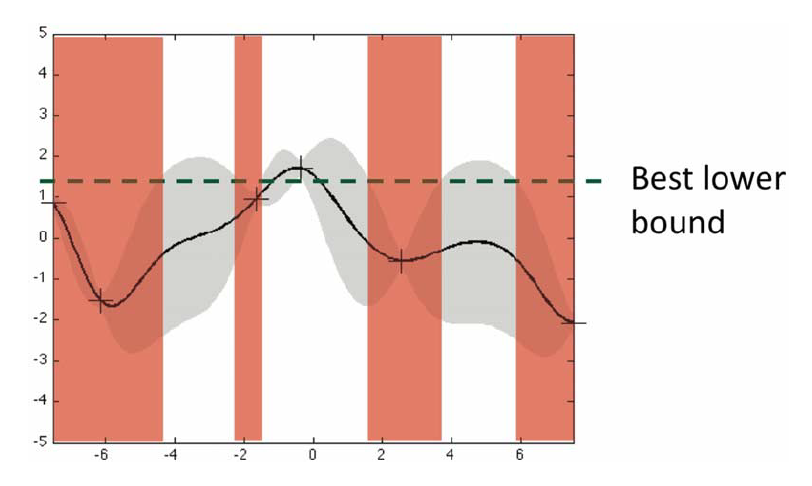
\includegraphics[width=\columnwidth]{fig/GPUCB.png}
    \captionof{figure}{GP-UCB selection rule rules out regions of the decision set where the upper confidence bound is less than the maximum lower confidence bound. \cite{srinivas2012}}
    \label{fig:3settings}
\end{center}\\
\textbf{Quantile Regression}: The $\tau$th quantile of random variable Y
$$Q(\tau) = \inf\{y: F(y) \geq \tau\}$$
The quantiles can be formulated as the solution to a optimization problem. For any $0 < \tau < 1$, define pairwise linear "check function" as following \cite{koenker2001quantile}
$$\rho_\tau(u) = u(\tau - I(u<0))$$
\begin{center}
    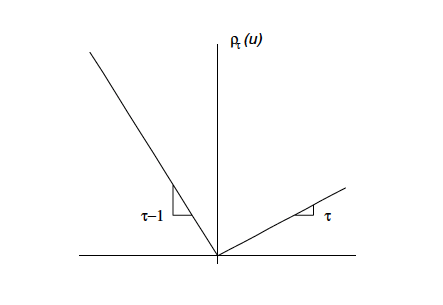
\includegraphics[width=\columnwidth]{fig/quant.png}
    \captionof{figure}{Quantile Regression Optimization Function \cite{koenker2001quantile}}
    \label{fig:quant}
\end{center}\\
\section{Ideas}
\vspace{-.6cm}

Instead of model $f$ with the strong assumption of Gaussian Process, we can rely on quantile regression to estimate the upper confidence bound. We propose Quantile Regression Upper Confidence Bound (Quant-UCB), which uses quantile (e.g. 85\%) instead of Gaussian variance. \\
 
\begin{itemize}
\item \ Directly using upper quantile. 
    $$x_t = \argmax_{x \in D} Q(\tau_{t-1})$$
    where $0 < \tau_{t-1} < 1$ and $\tau$ is proportional to iteration t.
\item \ Using median (50\% quantile) as rewards, the difference between upper quantile (e.g. 90\%) and lower quantile (e.g. 10\%) as uncertainty. 
$$x_t = \argmax_{x \in D} mq_{t-1} (x) + \beta_t^{1/2} (uq_{t-1} (x) - lq_{t-1}(x))$$
When using multiple quantiles, quantile functions are likely to cross, and thus violating the basic principle that the cumulative distribution function should be monotonically non-decreasing. One can use joint quantile regression in vector-valued RKHSs to avoid this crossing problem \cite{Sangnier:2016:JQR:3157382.3157511}. 
\end{itemize}
%\columnbreak

%----------------------------------------------------------------------------------------
% column 2: methods
%----------------------------------------------------------------------------------------
\section{Open Questions}
\textmoveup

\begin{itemize}
    \item Does cumulative regret bounds exist for Quant-UCB? If so, how to prove the regret bound theoretically? 
    \item Compared with GP-UCB, what advantages and disadvantages does Quant-UCB have? In other words, under what constraints or for what kind of data, Quant-UCB performs better?
    \item What optimization algorithm we should use for Quant-UCB? For example, one choice could be making use of stochastic sub-gradient descent (SSGD) to perform sequential optimization; another possibility is to use dual optimization for joint quantile regression, as proposed in \cite{Sangnier:2016:JQR:3157382.3157511}.
    \item How to measure the performance of the proposed algorithm? i.e. how do we know Quant-UCB can beat related algorithms under some certain constraints? By measuring cumulative regret? efficiency? 
\end{itemize}

\section{Experiment}

\begin{center}
    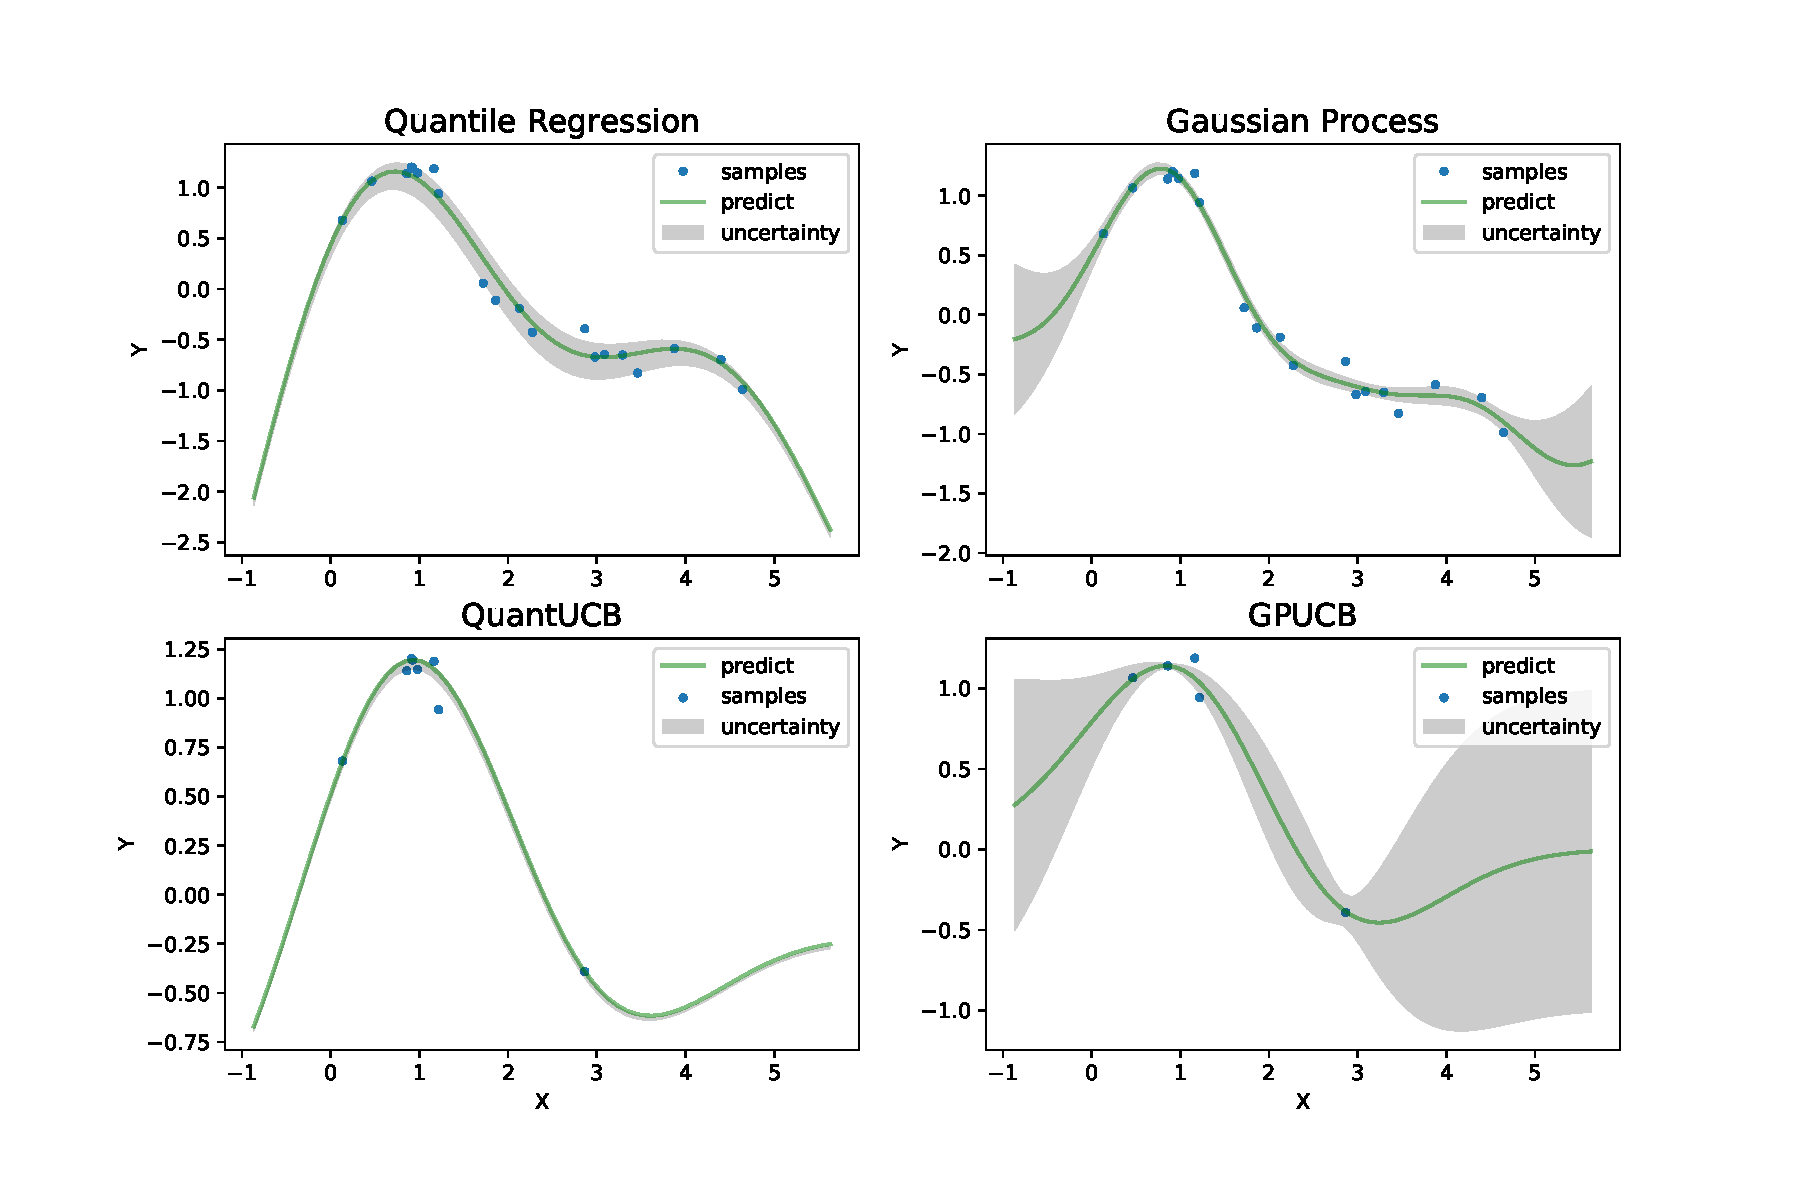
\includegraphics[scale=1.2]{fig/Exper.pdf}
    \captionof{figure}{Experiments on toy data. The first row shows quantile regression and Gaussian Process regression fitting. The second row shows the selected samples for Quant-UCB and GP-UCB respectively.} 
    \label{fig:quant}
\end{center}


\printbibliography
\end{multicols}
\end{document}
